\begin{figure*}[!htb]
\centering
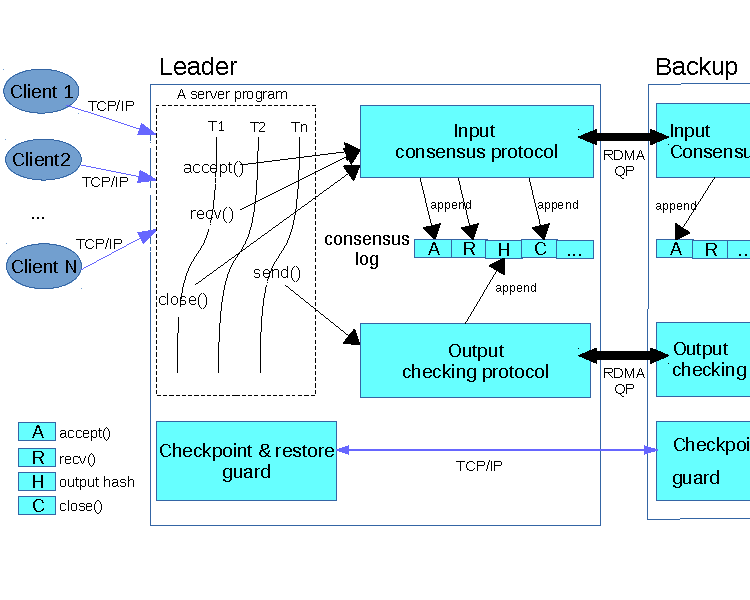
\includegraphics[width=1\textwidth]{figures/arch}
\vspace{-.10in}
\caption{{\em The \xxx Architecture.} \rm {\xxx components are shaded (and in
  green).}} \label{fig:arch}
\vspace{-.05in}
\end{figure*}

\section{\xxx Overview}\label{sec:overview}

As concurrency attacks raised many security challenges and the concurrency 
errors that can lead to these attacks are hidden in the excessive number of 
reports, we build \xxx, an automated concurrency attack detection 
framework. This section presents an overview of \xxx's architecture with main 
components and workflow (\S\ref{sec:arch}), and it gives an example to show how 
it works (\S\ref{sec:example}).



\subsection{Architecture}\label{sec:arch}

Figure~\ref{fig:arch} presents \xxx's architecture with three key components: 
the concurrency error detector (for short, \emph{detector}), the false positive 
filter (\emph{filter}), and the security consequence analysis tool 
(\emph{analyzer}). \xxx takes both program source code and inputs, and it 
outputs real or potential reports of concurrency attacks. This project 
targets open source C/C++ programs. Program inputs can be popular workloads or 
developer test suites of these programs.

The detector takes a program's inputs and executable and outputs concurrency 
error reports. This paper leverages \tsan~\cite{tsan:wbia09} for 
application programs and \ski~\cite{ski:osdi14} for kernels. We chose these two 
detectors because they are both open source, popular, and have shown to detect 
harmful bugs in many large programs. We modified these two detectors to match the 
input formats for our filter and analyzer (\S\ref{sec:tool}).

As presented in our study, one common issue in existing concurrency bug 
detectors is that their reports are typically enormous and deeply 
bury the vulnerable ones. Most of these reports are not even harmful, regular 
concurrency bug, thus passing all these reports to \xxx's analyzer is time 
consuming and helpless on detecting concurrency attacks.

To address this issue, our filter component takes both the detector's reports 
and LLVM bitcode to filter out harmless reports. Our filter currently handles 
four types of benign reports, including duplicate call stack reports, 
semaphore-like ad-hoc synchronizations, bit operations, and customized mutex 
operations. In our evaluation, these filter types are already sufficient to 
prune most of false positives from the detector without missing harmful ones.
% , and more types can be added.

Our analyzer component takes the remaining, potentially vulnerable reports from 
the filter, and does static analysis on the LLVM bitcode to identify potential 
security consequence of each report. The analyzer starts from the first LLVM 
\v{load} (memory read) instruction on a bug report's corrupted memory and does 
inter-procedural analysis on how this corrupted read value propagates through 
data flows and control flows. To achieve scalability to large programs, the 
analyzer does the propagation analysis \wrt current call stack of the 
read instruction. More details on the analyzer will be given in 
\S\ref{sec:algo}.

\subsection{Example}\label{sec:example}
% 
% We'll use an example to demonstrate how \xxx's components work together to
% detect a real world concurrency attack.
% \libsafe is 

Figure~\ref{fig:libsafe} shows a concurrency attack in \libsafe, a user-level 
security library that intercepts all the Libc memory functions to detect buffer 
overflows. When \libsafe detects a buffer overflow, it sets a global variable 
\v{dying} to 1 to indicate that current process will be killed shortly, and 
then it kills the program. If this variable is set, \libsafe will stop to 
perform security checks on memory functions. Unfortunately, there is a data 
race on \v{dying} because acess to this variable is not protected by mutex. 
Therefore, between the moment \v{dying} is set and the moment the entire process 
is killed, a thread calling memory functions in this process may leverate the 
race on \v{dying} to bypass buffer overflow checks.

We have constructed a C program with \libsafe to trigger this race, bypassed a 
stack overflow check for a vulnerability site, \v{strcpy()}, and got a shell by 
injecting our own malicious code. Note that in this attack, the race and the 
vulnerability site are in different functions, and the race affects the 
vulnerability site through an \v{if} control-dependency at line 164. Existing 
analysis tools~\cite{conseq:asplos11,yamaguchi:sp14,livshits05finding} are 
inadequate to detect this attack because they lack either inter-procedural or 
control-flow analysis.

\xxx detects the concurrency attack in this program with three steps. First, we 
use our C program to ``accidentally'' write across the memory boundary, thus 
\v{dying} is set. \xxx's concurrency bug detector \tsan detects a data race on 
\v{dying} and generates a race report. Second, all our four filters pass this 
report and consider it as harmful because this report matches none of the three 
types of false positive filters we provide (\S\ref{sec:impl}).

Third, \xxx's analyzer starts from the race's call stack shown in 
Figure~\ref{fig:call_stack}, and it conducts a inter-procedural static analysis 
to detect which vulnerability site may be affected by this race by tracking 
data and control flows. As shown in Figure~\ref{fig:libsafe_result}, \xxx 
reported one memory operation at line 165 as a potential vulnerability site. 
Combining with the race, line 165 indicates that a \v{strcpy()} function will be 
called with the original parameters without the actual security checks in 
\v{stack\_check()}. \xxx's analyzer reports this potential vulnerabilities are 
control-dependent on the branch statement at line 164. By learning from this 
report, we further crafted the C program with two busy loops calling 
\v{libsafe\_strcpy()}, and then our program easily triggered this attack with 
only a few repetitive executions. 

\begin{figure}
  \centering
  \lstset{basicstyle=\ttfamily\fontsize{6}{6}\selectfont,
  morekeywords={_bytes,_sumbytes}}
  \mbox{\lstinputlisting[mathescape,boxpos=t]{code/libsafe_callstack.txt}}
  \vspace{-.1in}
  \caption{{\em \libsafe call stack}. \rm {Line numbers refer to 
Figure~\ref{fig:libsafe}.}
  }
%   \vspace{-.1in}
  \label{fig:call_stack}
\end{figure}


\begin{figure}
  \centering
  \lstset{basicstyle=\ttfamily\fontsize{6}{6}\selectfont,
  morekeywords={_bytes,_sumbytes}}
  \mbox{\lstinputlisting[mathescape,boxpos=t]{code/libsafe_result.txt}}
  \vspace{-.1in}
  \caption{{\em \xxx detection result on the \libsafe attack.} \rm {Line 
numbers refer to Figure~\ref{fig:libsafe}.} 
  \vspace{-.2in}
  }
  \label{fig:libsafe_result}
\end{figure}

% 
% TBD: heming, ephasis we are inter-procedural, capture indirect control flow 
% propagation.

%The example needs to show two benefits: with the bug report only, but the 
%vulnerability did not triggered in the detector's run, but with our backend 
%report, we idenfied those critical branches and function calls, refined our 
%workloads, and then triggered this attack. And we can trigger this attack with 
%only few executions.

% Our design adheres to the following goals.
